\documentclass[tikz,border=2pt]{standalone}
\usepackage[T1]{fontenc}
\usepackage{lmodern}
\usepackage{amsmath}
\usetikzlibrary{arrows.meta}

% Color supplements the component labels; it is not needed to identify them.
\definecolor{compA}{HTML}{0072B2}
\definecolor{compB}{HTML}{D55E00}
\definecolor{compC}{HTML}{009E73}
\definecolor{compD}{HTML}{CC79A7}
\newcommand{\figtext}{\fontsize{9}{11}\selectfont}
\newcommand{\figlabel}{\fontsize{10}{12}\selectfont}

% A triangle denotes a fixed rooted component, with its attachment at the apex.
% Arguments: horizontal position, then four component-id/color pairs.
\newcommand{\fullquartet}[5]{%
 \begin{scope}[shift={(#1,4.15)}]
  \draw[tree] (-.36,0)--(.36,0);
  \foreach \x/\y/\id/\col in
    {-1/.56/#2, -1/-.56/#3, 1/.56/#4, 1/-.56/#5}{
   \pgfmathsetmacro{\side}{ifthenelse(\x<0,-.36,.36)}
   \pgfmathsetmacro{\base}{ifthenelse(\y<0,\y-.61,\y+.61)}
   \pgfmathsetmacro{\mid}{(\y+2*\base)/3}
   \draw[tree] (\side,0)--(\x,\y);
   \filldraw[draw=\col,fill=\col!16,line width=.7pt]
     (\x,\y)--(\x-.37,\base)--(\x+.37,\base)--cycle;
   \fill[black!80] (\x,\y) circle (1pt);
   \node[font=\figlabel,inner sep=0pt] at (\x,\mid) {$S_{\id}$};
  }
  \fill[black!80] (-.36,0) circle (1.3pt);
  \fill[black!80] (.36,0) circle (1.3pt);
 \end{scope}}

\newcommand{\skeleton}[5]{%
 \begin{scope}[shift={(#1,4.15)}]
  \draw[tree] (-.36,0)--(.36,0);
  \foreach \x/\y/\id/\col in
    {-1/.82/#2, -1/-.82/#3, 1/.82/#4, 1/-.82/#5}{
   \pgfmathsetmacro{\side}{ifthenelse(\x<0,-.36,.36)}
   \draw[tree] (\side,0)--(\x,\y);
   \node[circle,draw=\col,fill=\col!16,line width=.7pt,
       minimum size=6mm,inner sep=1.6pt,font=\figlabel]
       at (\x,\y) {$S_{\id}$};
  }
  \fill[black!80] (-.36,0) circle (1.3pt);
  \fill[black!80] (.36,0) circle (1.3pt);
 \end{scope}}

\begin{document}
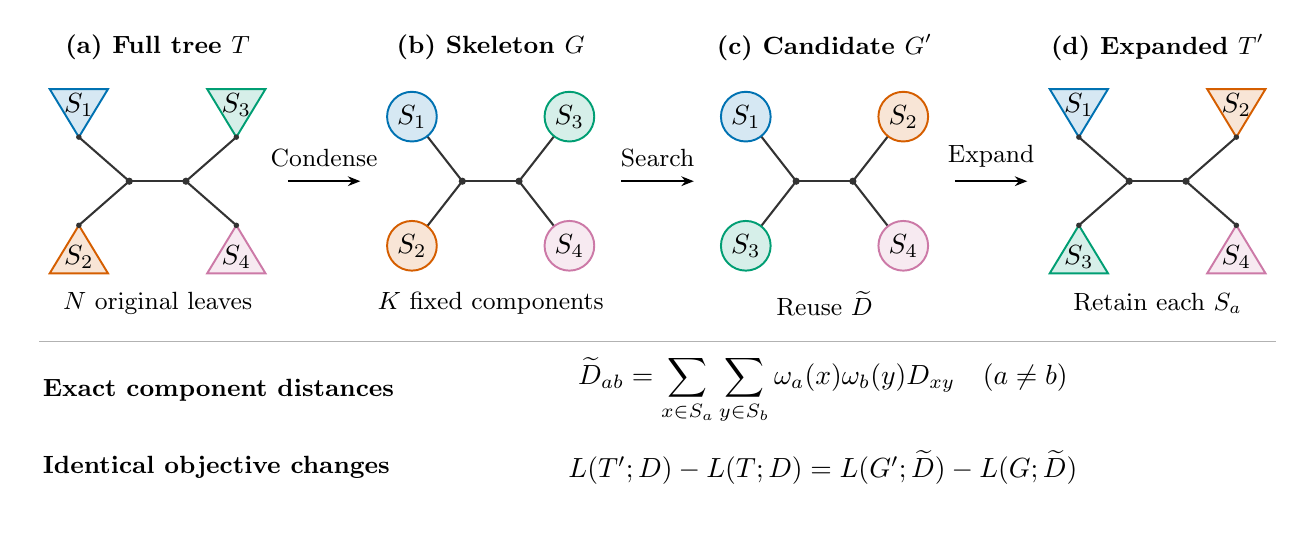
\begin{tikzpicture}[
 tree/.style={line width=.75pt,draw=black!80},
 >={Stealth[length=4.5pt,width=3.5pt]},
 every node/.style={text=black,inner sep=1pt}]
 % Designed for a full text-width figure, approximately 162--170 mm wide.
 \path[use as bounding box] (0,0) rectangle (16,6.1);

 \fullquartet{1.65}{1/compA}{2/compB}{3/compC}{4/compD}
 \skeleton{5.88}{1/compA}{2/compB}{3/compC}{4/compD}
 \skeleton{10.12}{1/compA}{3/compC}{2/compB}{4/compD}
 \fullquartet{14.35}{1/compA}{3/compC}{2/compB}{4/compD}

 \foreach \x/\letter/\name in
   {1.65/a/{Full tree $T$},5.88/b/{Skeleton $G$},
    10.12/c/{Candidate $G'$},14.35/d/{Expanded $T'$}}{
   \node[font=\figtext\bfseries] at (\x,5.85) {(\letter) \name};
 }

 \foreach \x/\name in {3.765/Condense,8/Search,12.235/Expand}{
   \draw[->,line width=.7pt] (\x-.46,4.15)--(\x+.46,4.15);
   \node[font=\figtext,anchor=south] at (\x,4.29) {\name};
 }
 \node[font=\figtext] at (1.65,2.6) {$N$ original leaves};
 \node[font=\figtext] at (5.88,2.6) {$K$ fixed components};
 \node[font=\figtext] at (10.12,2.6) {Reuse $\widetilde D$};
 \node[font=\figtext] at (14.35,2.6) {Retain each $S_a$};

 \draw[black!30,line width=.4pt] (.15,2.12)--(15.85,2.12);
 \node[font=\figtext\bfseries,anchor=west] at (.15,1.5)
    {Exact component distances};
 \node[font=\figlabel] at (10.1,1.5)
    {$\displaystyle\widetilde D_{ab}
      =\sum_{x\in S_a}\sum_{y\in S_b}\omega_a(x)\omega_b(y)D_{xy}
      \quad(a\ne b)$};
 \node[font=\figtext\bfseries,anchor=west] at (.15,.52)
    {Identical objective changes};
 \node[font=\figlabel] at (10.1,.52)
    {$L(T';D)-L(T;D)=L(G';\widetilde D)-L(G;\widetilde D)$};
\end{tikzpicture}
\end{document}
